\section{Case Study}
\label{sec:case-study}

We consider a multi-hop network which has a chain of OpenWSN nodes (see Figure~\ref{fig:multihop}), where each node has a different {\em NodeId} (assigned as an integer), increasing from left to right. 
\begin{figure}[t]
\centering
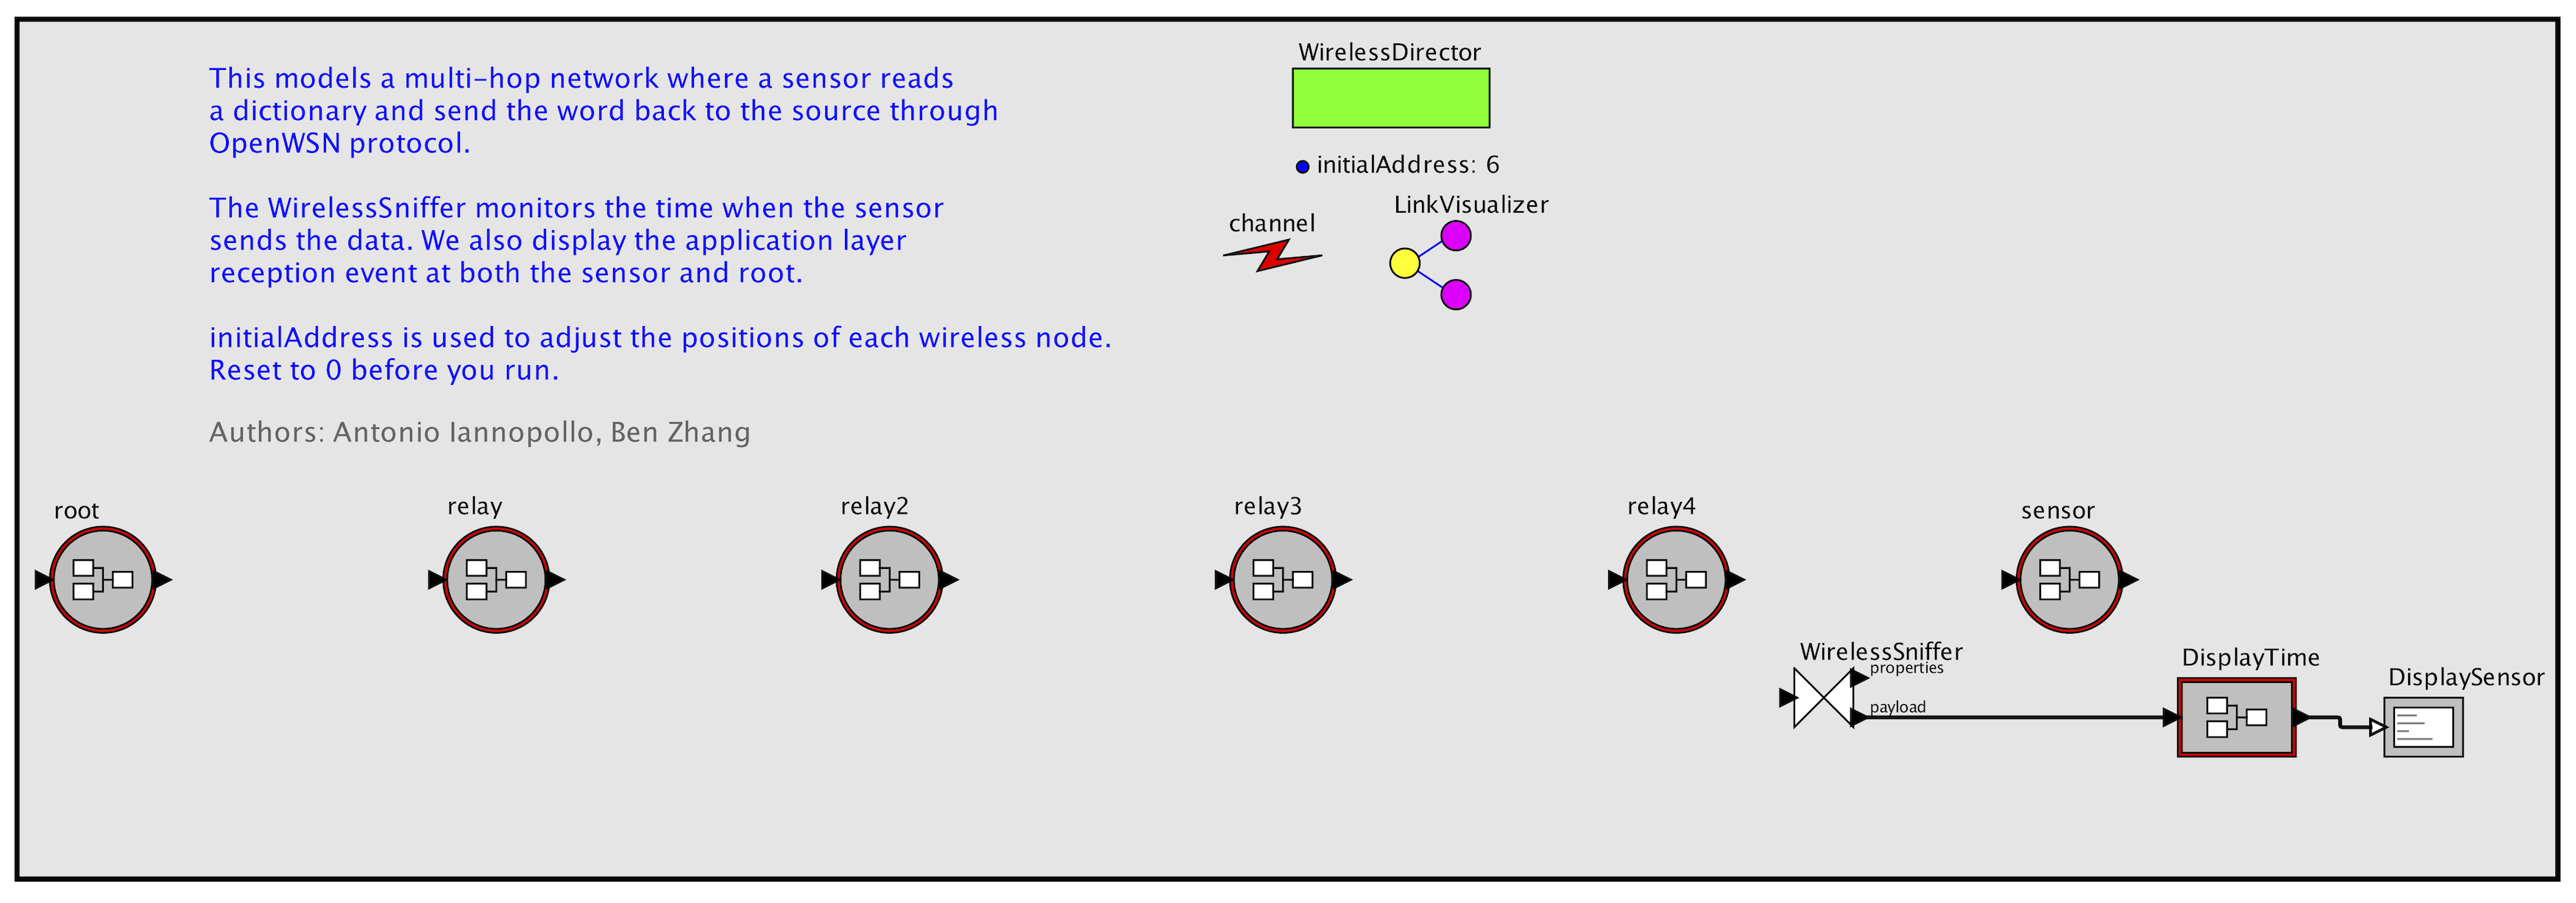
\includegraphics[width=1\columnwidth]{figures/PaperDemoPtolemy}
\caption{A multi-hop OpenWSN network.}
\label{fig:multihop}
\end{figure}
Node schedules are constructed following the schema\footnote{Interestingly, we are inspired by Gustove function to came up with such a schedule so that at any given time, a node is communicating only with one of its neighbors such that there will not be hidden terminal problem if time synchronization is achieved.}:

\begin{tabular}{ l | c | c | c | c | c }
  \hline                       
  NodeId & \multicolumn{5}{c}{Schedules} \\
  \hline
  $3i+0$ & \texttt{ADV} & \texttt{TX} & \texttt{RX} & \texttt{OFF} & $k \times \texttt{OFF}$ \\
  $3i+1$ & \texttt{ADV} & \texttt{RX} & \texttt{OFF} & \texttt{TX} & $k \times \texttt{OFF}$ \\
  $3i+2$ & \texttt{ADV} & \texttt{OFF} & \texttt{TX} & \texttt{RX} & $k \times \texttt{OFF}$ \\
  \hline  
\end{tabular}
where $i \in \mathbb{N}$ and $k$ is specified to control the duty cycle of each node (higher $k$ indicates more \texttt{OFF} in the schedule period and thus a lower duty cycle). Intuitively, when $k$ is small, nodes can receive \texttt{ADV} packet in a relatively timely fashion. This helps especially in case of lost synchronization. However, in case of high duty cycle schedules, the price a node needs to pay is to spend more time in \texttt{TX} and \texttt{RX} states, which potentially increases the power consumption. On the other hand, if $k$ is large, nodes that have lost synchronization will have to wait longer, leading to an increased energy consumption caused by turning the radio on and listening for long periods. Schedule duty cycle tuning is a critical activity in order achieve performance while minimizing energy consumption. In this work, we leave a formal study as future work, and only focus on cases when $k = 0, 144, 306$.

\begin{figure}
\hfill
\subfigure[For each node, the time it first get synchronized (the time it joins the network).]{ 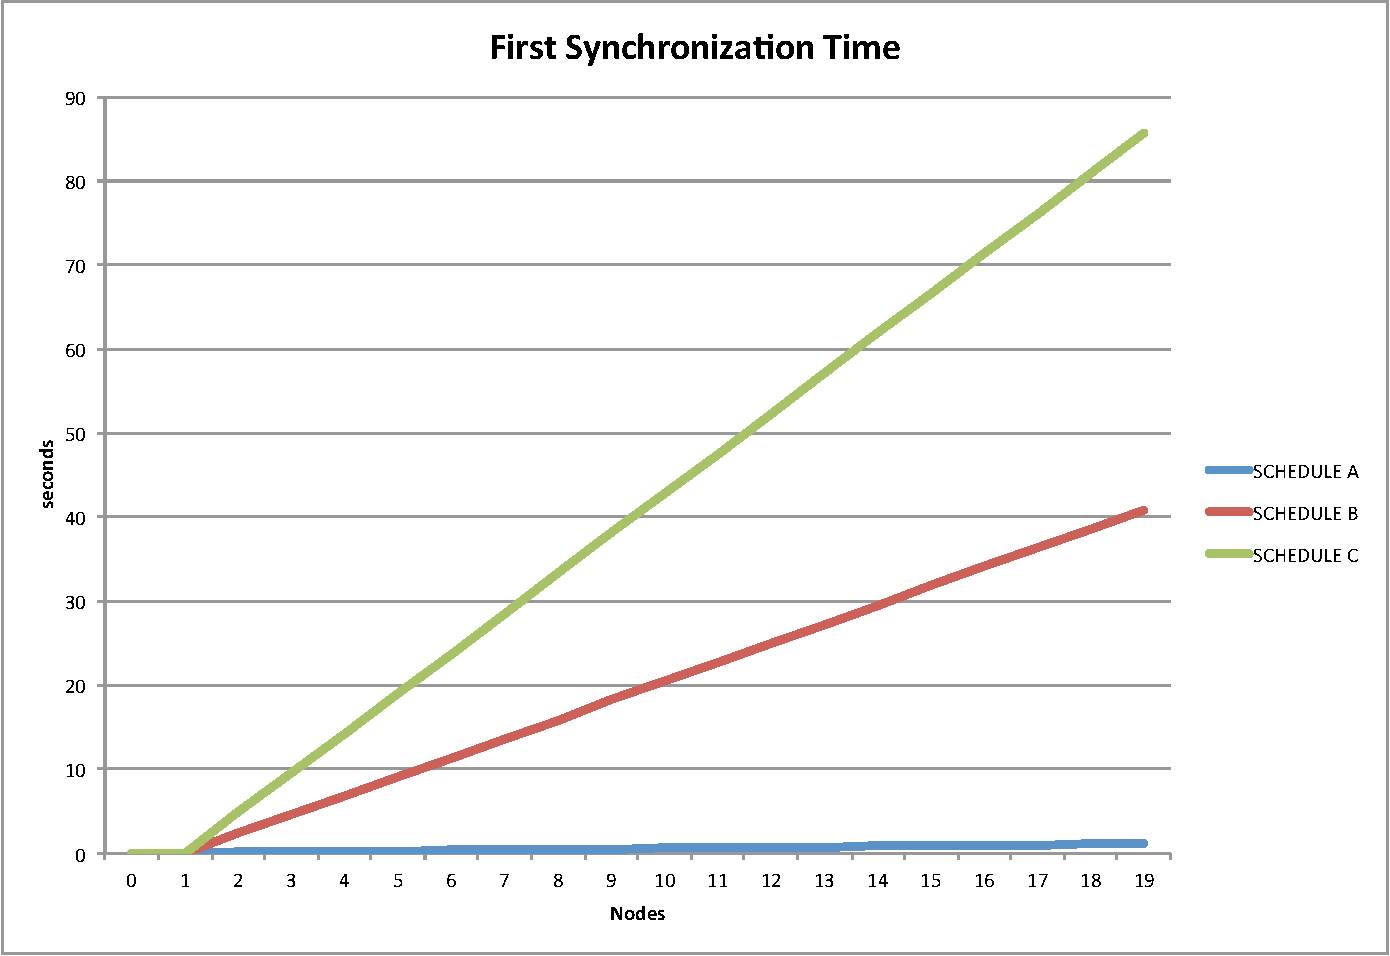
\includegraphics[width=.45\linewidth]{figures/synch_time_sched}}
\hfill
\subfigure[For each node, the measured power consumption after then network is on for 20 seconds.]{ 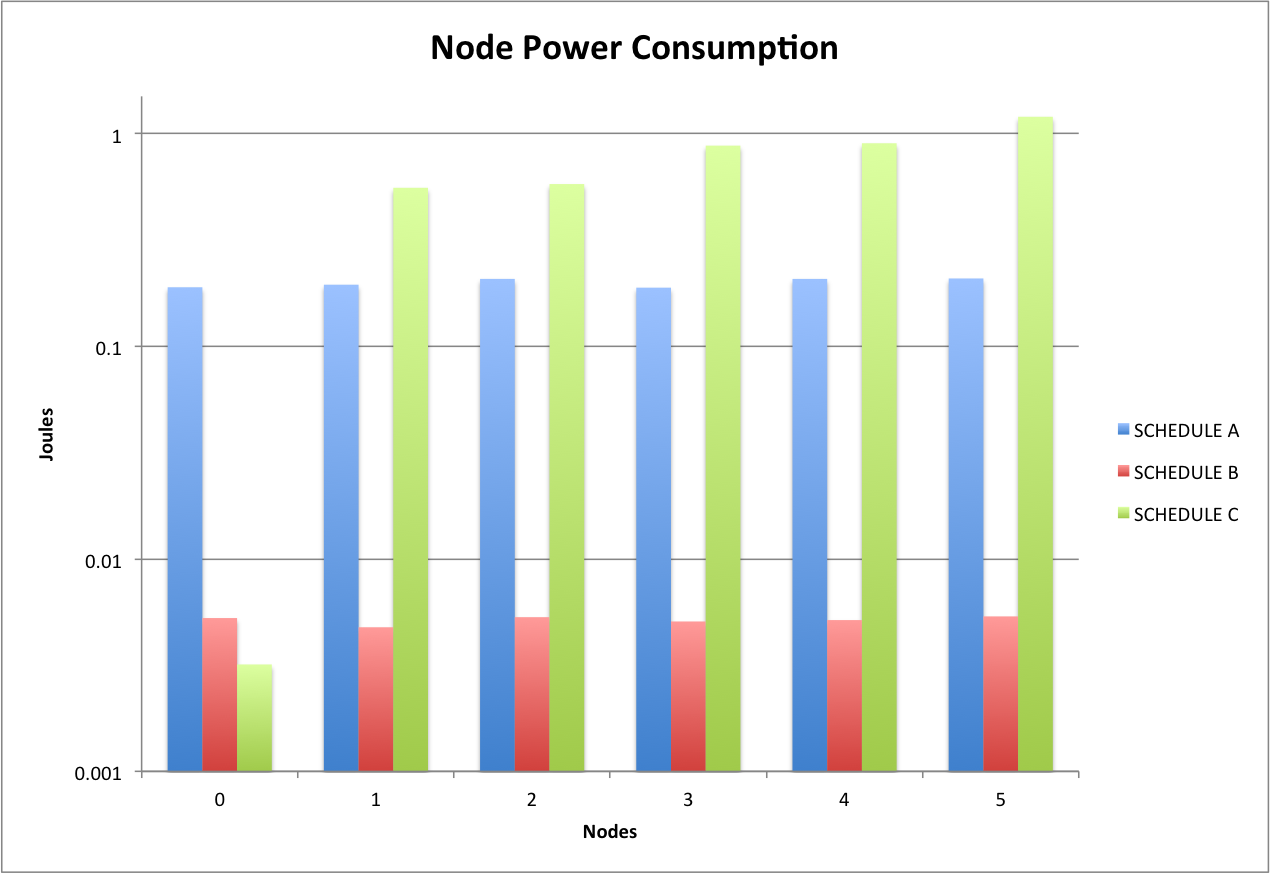
\includegraphics[width=.45\linewidth]{figures/power_cons}}
\hfill
\caption{Performance evaluation for different schedules in a multi-hop network. Schedule A, B, C are corresponding to $k = 0, 144, 306$.}
\label{fig:evaluation}
\end{figure}

We present the results of a network that has 6 chained nodes\footnote{The first synchronization figure was obtained with a simulation of 20 nodes. Given that the linear relationship is clear, we present the graph with 6 nodes for consistency with the power consumption results.} under the three different schedules in Figure~\ref{fig:evaluation}; and use two metrics to evaluate each schedule. The first metric is the time of first synchronization for each node in the network. This metric gives us an idea of how \emph{reactive} the network is. The second is the power consumption of each node in the network for a given period of time. This helps to evaluate the overall lifetime of network devices, which correlates to the network {\em durability}.

Keeping looking at Figure~\ref{fig:evaluation}, on the left, we see that the first synchronization time is proportional to the relative distance of each node from the root (as the reader intuition suggests). In case of higher duty cycle, when $k$ is smaller (such as with Schedule A), each node waits for a shorter time to reach synchronization. 

From the power consumption side (figure on the {\em right}), we have found that if the duty cycle is high ($k$ is small), then most nodes are busy in \texttt{TX} and \texttt{RX} states, leading to similar energy consumption values. When the duty cycle is low, then nodes that are farther from the root tend to stay longer in the \texttt{synchronization} state (because of the less frequent \texttt{ADV} packets), resulting in longer times with the radio in listening mode. Interestingly, schedules with a moderate duty cycle (see Schedule B), where transmissions are less frequent but not in a way to cause node de-synchronization, lead to an overall smaller amount of energy consumption. 

%%% Local Variables: 
%%% mode: latex
%%% TeX-master: "ee219d"
%%% End: 
